\documentclass[a4paper]{jpconf}
\usepackage{graphicx}
\usepackage{hyperref}
\usepackage{amssymb,amsfonts} % AMS Symbols
\usepackage{bm} % bold math

\hypersetup{pdftitle={SageManifolds},
  colorlinks=true
}

\newcommand{\soft}[1]{\texttt{#1}}
\newcommand{\code}[1]{\texttt{#1}}
\newcommand{\Sage}{\soft{Sage}}
\newcommand{\SM}{\soft{SageManifolds}}
\newcommand{\be}{\begin{equation}}
\newcommand{\ee}{\end{equation}}
\newcommand{\w}[1]{\bm{#1}}

\begin{document}
\title{Tensor calculus with free software: \\
the SageManifolds project}

\author{Eric Gourgoulhon$^1$, Micha\l{} Bejger$^2$, Marco Mancini$^1$}

\address{$^1$ Laboratoire Univers et Th\'eories, UMR 8102 du 
CNRS, Observatoire de Paris, Universit\'e Paris Diderot,
92190 Meudon, France}

\address{$^2$ Centrum Astronomiczne im. M. Kopernika, ul. Bartycka 18,
00-716 Warsaw, Poland}

\ead{eric.gourgoulhon@obspm.fr}

\begin{abstract}
Abstract
\end{abstract}

\section{Introduction}

Computer algebra for general relativity (GR) has a long history, which started
almost as soon as computer algebra itself in the 1960s. 
The first GR software was \soft{ALAM} (for \emph{Atlas Lisp Algebraic Manipulator})
witten by R.A. d'Inverno in 1969; he used it to compute
the Riemann and Ricci tensors of the Bondi metric.
According to \cite{Skea94}, 
the original calculations took Bondi and his collaborators 6 months to go,
while the computation with \soft{ALAM} took 4 minutes and yield to the 
discovery of 6 errors in the original paper. 
Since then, many packages have been developed and the reader is refered to \cite{MacCa02}
for a review of computer algebra
systems for GR prior to 2002 and to \cite{KorolKS13} for a more recent review,
focussing on tensor calculus. 
It is also worth to point out the quasi-exhaustive list of
tensor calculus packages maintained by J. M. Martin-Garcia at \cite{xact_links}.

%%%%%%%%%%%%%%%%%%%%%%%%%%%%%%

\section{Software for differential geometry}

Software packages for differential geometry and tensor calculus can be 
classified in two categories: 
\begin{enumerate}
\item Applications atop some general purpose computer algebra system; 
notable examples are 
the \soft{xAct} suite \cite{Marti08,xAct} and \soft{Ricci} \cite{Ricci}, both
running atop \soft{Mathematica},
\soft{DifferentialGeometry} \cite{AnderT12,DiffGeom} integrated into \soft{Maple}, and \soft{Atlas 2}
\cite{Atlas2} for \soft{Mathematica} and \soft{Maple}.
\item Standalone applications; recent examples are \soft{Cadabra}  (field theory) \cite{Peete07,Cadabra},
\soft{SnapPy} (topology and geometry of 3-manifolds) \cite{SnapPy} and
\soft{Redberry} (tensors) \cite{BolotP13,Redberry}.
\end{enumerate}
All applications listed in the second category are free (open-source) software. In
the first category, \soft{xAct} and \soft{Ricci} are also free software, but
they run atop a proprietary product, the sources of which are closed (\soft{Mathematica}). 

As far as tensor calculus is concerned, the above packages can be distinguished by 
the type of computation that they perform: abstract index manipulations 
(\soft{xAct/xTensor}, \soft{Ricci}, \soft{Cadabra}, \soft{Redberry})
or component calculus (\soft{xAct/xCoba}, \soft{DifferentialGeometry}, \soft{Atlas 2})
In the first category, tensor operations such as contraction or covariant differentiation 
are performed by manipulating the indices themselves rather than the components 
to which they correspond. In the second category, vector bases are explicitely 
introduced on the manifold and tensor operations are carried out on the components 
in a given basis.


%%%%%%%%%%%%%%%%%%%%%%%%%%%%%%

\section{An overview of Sage}

\Sage{} \cite{sage} is a free open-source mathematics software system, which is
based on the Python programming language. It makes use of 90 open-sources packages, 
among which \soft{Maxima} and \soft{Pynac} (symbolic calculations),
\soft{GAP} (group theory), 
\soft{PARI/GP} (number theory), \soft{Singular} (polynomial computations), 
and \soft{matplotlib} (high quality 2D figures). 
\Sage{} provides a uniform Python interface to all these packages; however, 
\Sage{} is much more than a mere interface: it contains a large and increasing part of 
original code (more than 750,000 lines of Python and Cython, involving 5344 classes). 
\Sage{} has been created in 2005 by W. Stein \cite{SteinJ05} and since
then its development has been sustained by more than a hundred researchers
(mostly mathematicians). Good introductory textbooks about \Sage{} are
\cite{JoyneS14,Zimme13,Bard15}. 
 
Apart from the syntax, based on Python and not on some specific script 
language, a difference between \Sage{} and \soft{Maple} or \soft{Mathematica}
is the use of the \emph{Parent/Element} scheme, which makes \Sage{} closer to 
actual mathematics. For instance, in \soft{Mathematica}, all objects 
are trees of symbols and the language is essentially a set of 
sophisticated rules to manipulate the symbols. On the contrary, in \Sage{}
each object has a given type (i.e. is an instance of a given Python class), 
and one distinguishes \emph{parent} types, which model mathematical
sets with some structure (e.g. algebraic structure), from \emph{element} types,
which model set elements. 
In particular, calculus rules on elements are determined by the algebraic
structure of their parents. Automatic conversion rules, called \emph{coercions},
prior to a binary operation, e.g. $x+y$ with $x$ and $y$ having different 
parents, are defined at the level of the parents.

%%%%%%%%%%%%%%%%%%%%%%%%%%%%%%%%%%%%%%%%%%%%%%%%%%%%%%%%%%%%%%%%%%%%%%%

\section{The SageManifolds project}

\subsection{Aim and scope}

\Sage{} is well developed in many areas of mathematics but there is
very little for differential geometry and tensor calculus.
The aim of \SM{} \cite{SM} is to introduce differential manifolds and tensor fields
in \Sage{}, and to do it in a coordinate-independent manner. 
More precisely, one should not to stick to a single coordinate patch
but should be able to introduce various coordinate charts
on a manifold. Tensor fields must be manipulated as such and not through 
their components with respect to a specific (possibly coordinate) vector frame. 

Basically the work amounts to creating new Python classes\footnote{Let us
recall that within an object-oriented programming language (as Python),
a \emph{class} is a structure to declare and store the
properties common to a set of objects; these properties 
are data (called 
\emph{attributes} or \emph{state variables}) and functions acting 
on the data (called \emph{methods}); a specific realization of an object 
within a given class is called an \emph{instance} of that class.},
 such as 
\code{Manifold}, \code{Chart}, \code{TensorField} or \code{Metric},
to implement them within the Parent/Element scheme and to 
code the relevant mathematical operations as class methods.
For instance the class \code{Manifold}, devoted to real smooth manifolds,
is a parent class, which means that it inherits from Sage native class \code{Parent}.
On the other hand, the class devoted to manifold points, \code{Point}, 
is an element class and therefore inherits from Sage native class 
\code{Element}.
This is illustrated by the inheritance diagram of Fig.~\ref{f:domain_classes}.
In this diagram, each class at the base of an arrow is a subclass (also
called \emph{derived class}) of the class at the arrowhead.

\begin{figure}
\begin{center}
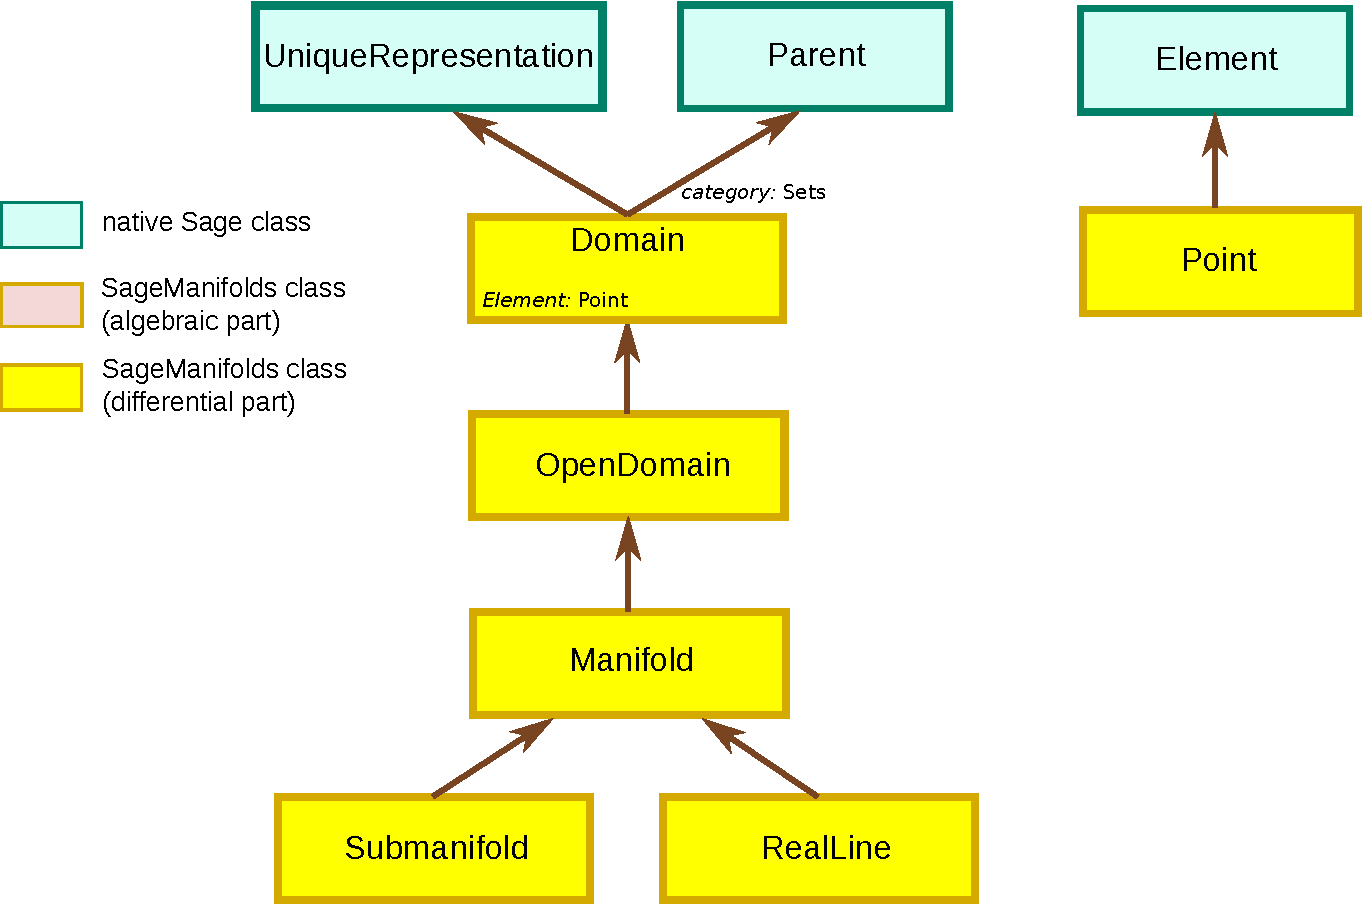
\includegraphics[width=0.7\textwidth]{domain_classes.pdf}
\end{center}
\caption{\label{f:domain_classes} Python classes for 
smooth manifolds (\code{Manifold}), generic subsets of them 
(\code{Domain}), open subsets of them (\code{OpenDomain})
and points on them (\code{Point}).}
\end{figure}

\subsection{Implementation of charts}

Given a manifold $\mathcal{M}$ of dimension $n$, a coordinate chart 
on an open subset $U\subset\mathcal{M}$ is implemented in \SM{} 
via the class \code{Chart}, whose main data is 
a $n$-uple of Sage symbolic variables $(x_1,\ldots,x_n)$, each of 
them representing a coordinate.
In general, more than one (regular) chart is required to cover the entire manifold.
For instance, at least 2 charts are necessary for the $n$-dimensional sphere 
$\mathbb{S}^n$ ($n\geq 1$), 3 charts for the real projective plane
$\mathbb{RP}^2$ and 4 charts for the torus $\mathbb{T}^2$.
Within \SM{}, an arbitrary number of charts can be introduced.
To fully specify the manifold, one shall also provide the transition maps
(changes of coordinates) on
overlapping chart domains (\SM{} class \code{CoordChange}).


\subsection{Implementation of scalar fields}

A \emph{scalar field} on manifold $\mathcal{M}$ is a smooth mapping
\be
    \begin{array}{lcll}
    f: & U\subset \mathcal{M}&\longrightarrow &\mathbb{R} \\
       & p & \longmapsto  & f(p) ,
    \end{array}
\ee
where $U$ is an open subset of $\mathcal{M}$.
Note that a scalar field maps \emph{points}, not \emph{coordinates}, to real numbers. 
A scalar field $f$ has different coordinate representations $F$, $\hat F$, etc. 
in different charts $C$, $\hat C$, etc. defined on $U$:
\be
    f(p) = 
F(\underbrace{x^1,\ldots, x^n}_{\mbox{coord. of $p$}\atop\mbox{in chart $C$}}) 
= {\hat F}(\underbrace{{\hat x}^1,\ldots, {\hat x}^n}_{\mbox{coord. of $p$}\atop\mbox{in chart $\hat C$}})
= \ldots
\ee
These representations are 
stored in an attribute of the class \code{ScalarField} that is a 
Python dictionary\footnote{A \emph{dictionary}, also known as \emph{associative array}, is a 
data structure that generalizes the concept of array in the sense that the
key to access to some element is not restricted to an integer or a tuple of integers.},
whose keys are the charts:
\be \label{e:f_express}
 f.\mbox{\texttt{\_express}} = \left\{ C: F,\ \hat C: \hat F, \ldots \right\} .
\ee

\begin{figure}
\begin{center}
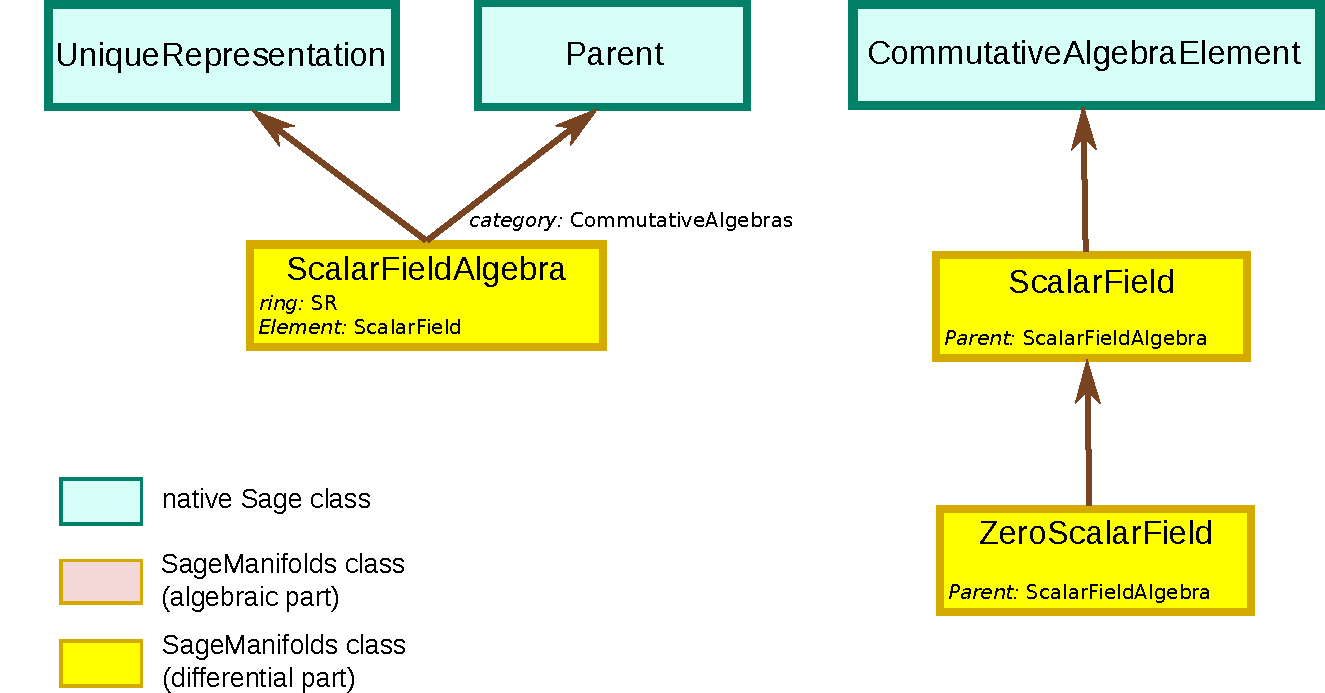
\includegraphics[width=0.7\textwidth]{scalar_classes.pdf}
\end{center}
\caption{\label{f:scalar_classes} Python classes for scalar fields
on a manifold.}
\end{figure}

Given an open subset $U\subset\mathcal{M}$, the set $C^\infty(U)$
of scalar fields defined on $U$ has naturally the structure of a 
commutative algebra over $\mathbb{R}$: it is clearly a vector
space over $\mathbb{R}$ and it is endowed with a commutative ring structure
by pointwise multiplication:
\be
\forall f, g \in C^\infty(U),\quad \forall p\in U,\quad
(f.g)(p) := f(p) g(p) .
\ee
The algebra $C^\infty(U)$ is implemented in \SM{} via the parent
class \code{ScalarFieldAlgebra}, the corresponding element class 
being \code{ScalarField} (cf. Fig.~\ref{f:scalar_classes}). 

\subsection{Modules and free modules} \label{s:modules}

Given an open subset $U\subset\mathcal{M}$, the set $\mathcal{X}(U)$
of all smooth vector fields defined on $U$ has naturally the structure of a 
module over the algebra $C^\infty(U)$.
Let us recall that a \emph{module} is similar to a \emph{vector space}, except that it is based
on a \emph{ring} (here $C^\infty(U)$)
instead of a \emph{field} (usually $\mathbb{R}$ or
$\mathbb{C}$ in physics). Of course, since every field is a ring, every vector space is a module.
There is an importance difference though: every vector space has a basis (as a 
consequence of the axiom of choice),
while a module does not necessarily have any. 
When it possesses one, it is called a \emph{free module}. 
Moreover if the module's base ring is commutative, all bases have the same
cardinality, which is called the \emph{rank} of the module 
(for vector spaces, which are free modules, the word \emph{dimension}
is used instead of \emph{rank}). 

If $\mathcal{X}(U)$ is a free module, a basis of it is nothing but a \emph{vector frame}
$(\w{e}_a)_{1\leq a \leq n}$ on $U$:
\be \label{e:v_expand}
    \forall \w{v}\in\mathcal{X}(U),\quad \w{v} = v^a \w{e}_a,\quad\mbox{with\ } v^a \in C^\infty(U) .
\ee
At any point $p\in U$, the above translates into an identity in 
the tangent vector space $T_p \mathcal{M}$:
\be 
    \w{v}(p) = v^a(p)  \; \w{e}_a(p),\quad\mbox{with\ } v^a(p) \in \mathbb{R} , 
\ee
which means that 
the set $(\w{e}_a(p))_{1\leq a \leq n}$ is a basis of the vector space $T_p \mathcal{M}$.
This is the very definition of a vector frame on $U$ (often called a \emph{tetrad} in
the context of 4-dimensional general relativity). Note that if $U$ is covered
by a chart $(x^a)_{1\leq a \leq n}$, then $(\partial/\partial x^a)_{1\leq a \leq n}$
is a vector frame on $U$, usually called \emph{coordinate frame}
or \emph{natural basis}. 

Another type of free modules which occur naturally in the current context
is that of the tangent spaces to the manifold $\mathcal{M}$: 
for each $p\in \mathcal{M}$, $T_p\mathcal{M}$ is a free module over 
$\mathbb{R}$, since it is a vector space over $\mathbb{R}$. 

It turns out that only free modules with a distinguished basis were 
implemented in \Sage{}. This means that, given a free module $M$ of rank $n$, 
all calculations refer a single basis of $M$. This amounts to identifying
$M$ with $R^n$, where $R$ is the ring over which $M$ is based. 
For dealing with generic manifolds in a coordinate-independent way, 
this is not appropriate. For instance, there is no canonical 
isomorphism between $T_p\mathcal{M}$ and $\mathbb{R}^n$ when no coordinate
system is privileged in the neightbourhood of $p$.
Therefore we have started a pure algebraic branch \SM{} to implement
generic free modules, with an arbitrary number of bases in them, 
none of them being distinguished. This resulted in the parent class 
\code{FiniteRankFreeModule} and in the element class 
\code{FiniteRankFreeModuleElement}. Then both the classes
\code{VectorFieldFreeModule} (for $\mathcal{X}(U)$ when it is 
a free module) and \code{TangentSpace} (for $T_p\mathcal{M}$)
inherit from \code{FiniteRankFreeModule} (see Fig.~\ref{f:module_classes}). 


\begin{figure}
\begin{center}
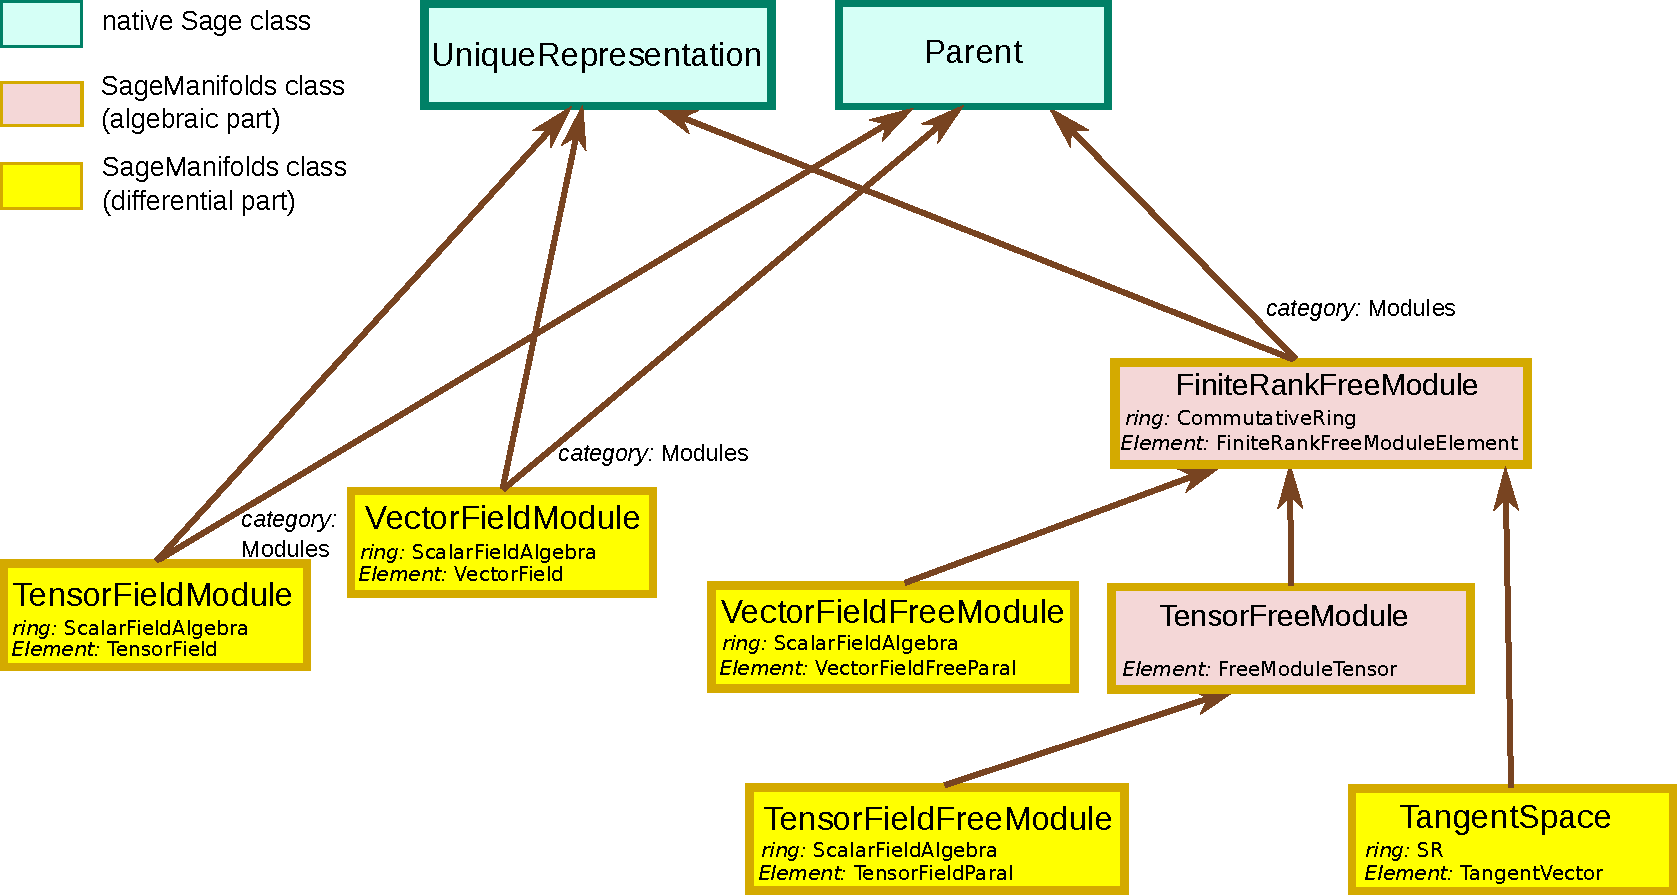
\includegraphics[width=0.8\textwidth]{module_classes.pdf}
\end{center}
\caption{\label{f:module_classes} Various module classes.}
\end{figure}



\subsection{Implementation of vector fields}

Ultimately, in \SM{}, vector fields are to be described by their 
components with respect to various vector frames, according to 
Eq.~(\ref{e:v_expand}), but without any vector frame being privileged, 
leaving the possibility to the user to change frames, as to change 
coordinates. A key point is that 
not every manifold admits a global vector frame. 
A manifold $\mathcal{M}$, or more generally an open subset $U\subset\mathcal{M}$,
that admits a global vector frame is called 
\emph{parallelizable}. Equivalently,
$\mathcal{M}$ is parallelizable if, and only if, $\mathcal{X}(\mathcal{M})$
is a free module. In terms of the tangent bundle, 
parallelizable manifolds are those for which the tangent bundle is trivial:
$T\mathcal{M} \simeq \mathcal{M}\times \mathbb{R}^n$.
Examples of parallelizable manifolds are \cite{Lee13}
\begin{itemize}
\item the Cartesian space $\mathbb{R}^n$ for $n=1,2,\ldots$; 
\item the circle $\mathbb{S}^1$; 
\item the torus $\mathbb{T}^2 = \mathbb{S}^1\times \mathbb{S}^1$;
\item the 3-sphere $\mathbb{S}^3 \simeq \mathrm{SU}(2)$, as any Lie group;
\item the 7-sphere $\mathbb{S}^7$ ; 
\item any orientable 3-manifold (Steenrod theorem \cite{Steen51}).
\end{itemize}
On the other hand, examples of non-parallelizable manifolds are
\begin{itemize}
\item the sphere $\mathbb{S}^2$ (hairy ball theorem!) and any $n$-sphere $\mathbb{S}^n$ with $n\not\in\{1,3,7\}$; 
\item the real projective plane $\mathbb{RP}^2$.
\end{itemize}
Actually, ``most'' manifolds are non-parallelizable. 
As noticed above, if a manifold is covered by a single chart, it is 
parallelizable (the prototype being $\mathbb{R}^n$). But the reverse is not 
true: $\mathbb{S}^1$ and $\mathbb{T}^2$ are parallelizable and require
respectively at least two and four charts to cover them. 

If the manifold $\mathcal{M}$ is not parallelizable, one has to decompose it 
into parallelizable
open subsets $U_i$ ($1\leq i \leq N$) 
and consider the restrictions of vector fields to these domains.
For each $i$, $\mathcal{X}(U_i)$ is a free module of rank $n=\mathrm{dim}\, \mathcal{M}$ and is implemented in \SM{} as an instance of 
\code{VectorFieldFreeModule} (cf. Sec.~\ref{s:modules} and Figs.~\ref{f:module_classes}
and \ref{f:tensor_classes}). 
Each vector field $\w{v}\in  \mathcal{X}(U_i)$ has different set
of components $(v^a)_{1\leq a\leq n}$ in different vector frames 
$(\w{e}_a)_{1\leq a \leq n}$ introduced on $U_i$ [cf. Eq.~(\ref{e:v_expand})]. They are stored
as a Python dictionary whose keys are the vector frames:
\be
\w{v}.\mbox{\texttt{\_components}} = \left\{ (\w{e}): (v^a),
\ (\w{\hat e}): ({\hat v}^a), \ldots \right\}. 
\ee

\begin{figure}
\begin{center}
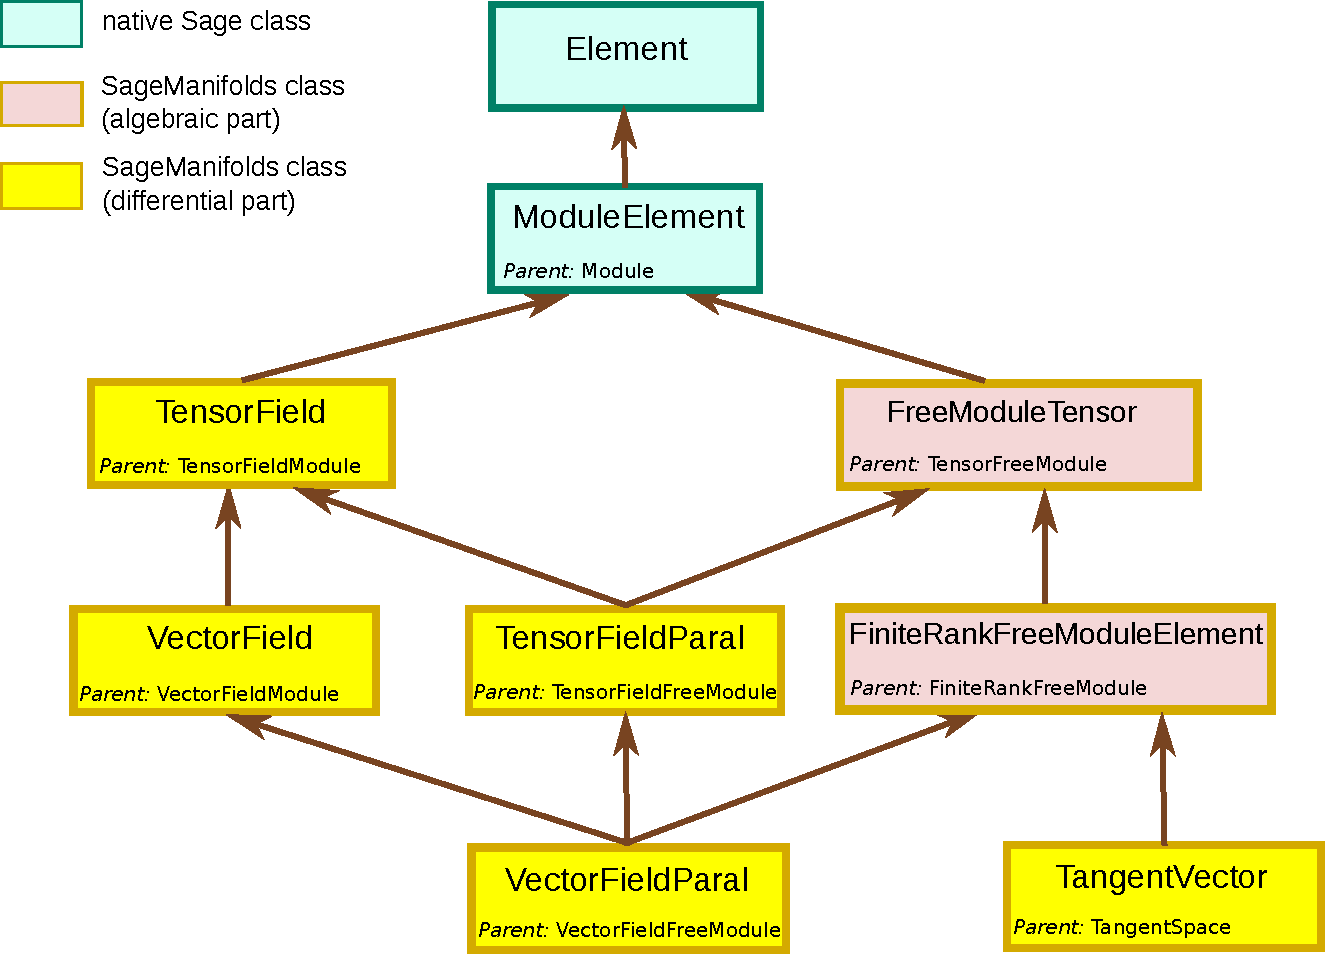
\includegraphics[width=0.7\textwidth]{tensorfield_classes.pdf}
\end{center}
\caption{\label{f:tensor_classes} Tensor and tensor field classes.}
\end{figure}


\subsection{Implementation of tensor fields}

The implementation of tensor fields in \SM{} follows the strategy 
adopted for vector fields. Consider for instance a tensor field $\w{T}$ 
of type-(1,1) on the manifold $\mathcal{M}$. 
It can be represented by 
components $T^a_{\ \, b}$ only on a parallelizable open subset $U\subset
\mathcal{M}$, since the decomposition 
\be \label{e:T_expand}
    \left. \w{T} \right| _{U} = T^a_{\ \, b} \, \w{e}_a \otimes \w{e}^b
\ee
defining $T^a_{\ \, b}$ is meaningfull only when a vector frame 
$(\w{e}_a)$ exist\footnote{Using standard notation, in Eq.~(\ref{e:T_expand})
$(\w{e}^b)$ stands for the coframe dual to $(\w{e}_a)$}.
Therefore, one first decompose the tensor field $\w{T}$  into 
its restrictions $\left. \w{T} \right| _{U_i}$ on parallelizable open subsets
of $\mathcal{M}$, $U_i$ ($1\leq i\leq N$) and then consider 
the components on various vector frames on each of the $U_i$'s. 
This is illustrated in Fig.~\ref{f:tensorfield_structure}, which details the
internal storage of tensor fields in \SM{}. Note that each component
$T^a_{\ \, b}$ is a scalar field on $U_i$, according to the formula
\be
    T^a_{\ \, b} = \w{T}(\w{e}^a, \w{e}_b) . 
\ee
Accordingly, at the last but one level of Fig.~\ref{f:tensorfield_structure}, 
there appears the scalar field storage, as decribed by (\ref{e:f_express}).
The last level is constitued by \Sage{}'s symbolic expressions. 

\begin{figure}
\begin{center}
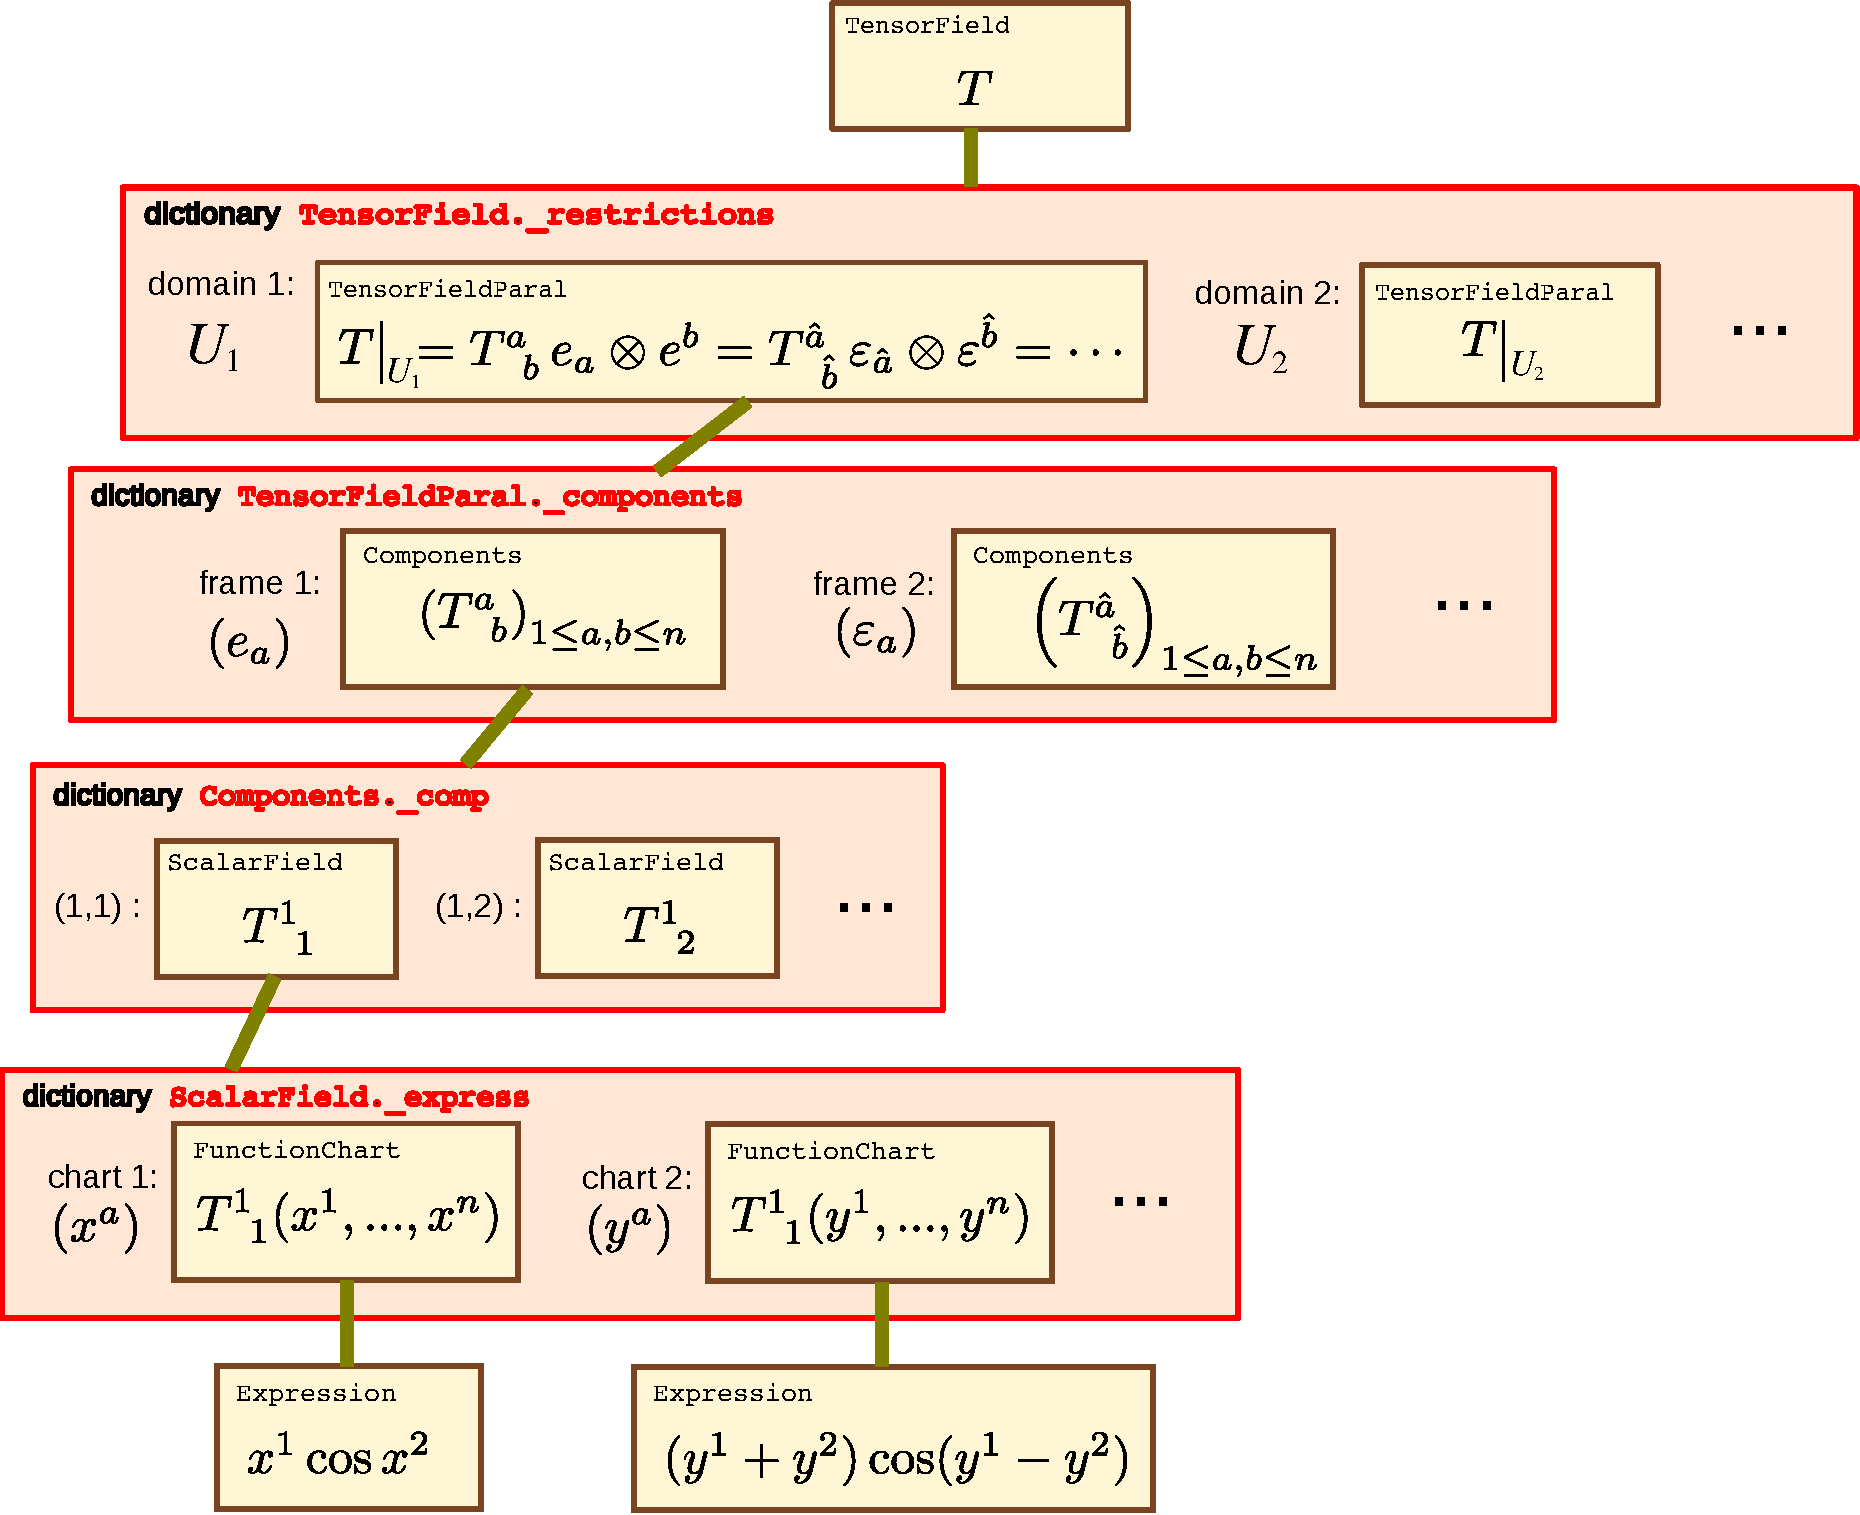
\includegraphics[width=0.8\textwidth]{tensorfield_structure.pdf}
\end{center}
\caption{\label{f:tensorfield_structure} Storage of tensor fields.}
\end{figure}



%%%%%%%%%%%%%%%%%%%%%%%%%%%%%%%%%%%%%%%%%%%%%%%%%%%%%%%%%

\section{Current status of SageManifolds}

\subsection{Functionalities}

At present, the functionalities included in \SM{} are 
\begin{itemize}
\item maps between manifolds, pullback operator
\item submanifolds, pushforward operator
\item standard tensor calculus (tensor product, 
contraction, symmetrization, etc.), even on non-parallelizable manifolds
\item all monoterm tensor symmetries 
\item exterior calculus, Hodge duality
\item Lie derivatives
\item affine connections, curvature, torsion
\item pseudo-Riemannian metrics, Weyl tensor
\end{itemize}


\subsection{Parallelization}

- Marco


%%%%%%%%%%%%%%%%%%%%%%%%%%%%%%%%%%%%%%%%%%%%%%%%%%%%%%%%%

\section{SageManifolds at work: the spacetime Simon tensor example}


%%%%%%%%%%%%%%%%%%%%%%%%%%%%%%%%%%%%%%%%%%%%%%%%%%%%%%%%%

\section{Conclusion and future propects}

- replacing SR (computation on a numerical spacetime)

\ack
This work has benifited from enlightening discussions with Volker Braun,
Vincent Delecroix, Simon King,  Jos\'e M. Mart\'\i n-Garc\'\i a, 
S\'ebastien Labb\'e,
Marc Mezzarobba, Thierry Monteil, Travis Scrimshaw and Nicolas Thi\'ery. 
We also thank St\'ephane M\'en\'e for his technical help. 
 


\section*{References}
\begin{thebibliography}{10}
\bibitem{Skea94}
Skea J E F 1994 Applications of SHEEP {\it Lecture notes available at}
\url{
http://www.computeralgebra.nl/systemsoverview/special/tensoranalysis/sheep/}
\bibitem{MacCa02}
MacCallum M A H 2002 {\it Int. J. Mod. Phys. A} {\bf 17}, 2707 
\bibitem{KorolKS13}
Korol'kova A V, Kulyabov D S and Sevast'yanov L A 2013 {\it Prog. Comput. Soft.} 
{\bf 39}, 135
\bibitem{xact_links} 
\url{http://www.xact.es/links.html}
\bibitem{Marti08}
Martin-Garcia J M 2008 {\it Comput. Phys. Commun.} {\bf 179}, 597
\bibitem{xAct}
\url{http://www.xact.es}
\bibitem{Ricci}
\url{http://www.math.washington.edu/~lee/Ricci/}
\bibitem{AnderT12}
Anderson I M and Torre C G 2012 {\it J. Math. Phys.} {\bf 53}, 013511
\bibitem{DiffGeom}
\url{http://digitalcommons.usu.edu/dg/}
\bibitem{Atlas2}
\url{http://digi-area.com/Maple/atlas/}
\bibitem{Peete07}
Peeters K 2007 {\it Comput. Phys. Commun.} {\bf 15}, 550
\bibitem{Cadabra}
\url{http://cadabra.phi-sci.com/}
\bibitem{SnapPy}
Culler M, Dunfield N M and Weeks J R, SnapPy, a computer program for studying the geometry and topology of 3-manifolds, \url{http://snappy.computop.org}
\bibitem{BolotP13}
Bolotin D A and Poslavsky S V 2013 Introduction to Redberry: the computer algebra system designed for tensor manipulation {\it Preprint} arXiv:1302.1219
\bibitem{Redberry}
\url{http://redberry.cc/}
\bibitem{sage}
\url{http://sagemath.org/}
\bibitem{SteinJ05}
Stein W and Joyner D 2005 {\it Commun. Comput. Algebra} {\bf 39}, 61
\bibitem{JoyneS14}
Joyner D and Stein W 2014 {\it Sage Tutorial} (CreateSpace)
\bibitem{Zimme13}
Zimmermann P et al. 2013 {\it Calcul math\'ematique avec Sage} (CreateSpace); 
freely downloadable from \url{http://sagebook.gforge.inria.fr/}
\bibitem{Bard15}
Bard G V 2015 {\it Sage for Undergraduates} (Americ. Math. Soc.) in press;
preprint freely downloadable from \url{http://www.gregorybard.com/})
\bibitem{SM}
\url{http://sagemanifolds.obspm.fr/}
\bibitem{Lee13}
Lee J M 2013 {\it Introduction to Smooth Manifolds} 2nd edition (New York: Springer)
\bibitem{Steen51}
Steenrod N 1951 {\it The Topology of Fibre Bundles} (Princeton: Princeton Univ. Press)
\end{thebibliography}

\end{document}
